\section{Related Work}
Image similarity is the measure of how similar two images are. One of the ways to build similarity model is to extract features such as SIFT \cite{van1999}, Local Binary Patterns, HOG \cite{dalal2005} and then use the features to compute the similarity between the features. Gabor filter is a linear filter used for texture analysis that analyzes whether there are any specific frequency content in the image in specific directions in a localized region around the point or region of analysis. Local binary patterns (LBP) is a type of visual descriptor used for classification in computer vision. We can also use deep learning model to identify images for a query image. The scale-invariant feature transform (SIFT) is a feature detection algorithm in computer vision to detect and describe local features in images. 
\vskip 5

Wang et al.\cite{wang2014learning} proposes a deep ranking model that employs deep learning techniques to learn similarity metric directly from images. It has higher learning
capability than models based on hand-crafted features. A multiscale network structure was developed to describe the images effectively. An efficient triplet sampling algorithm is proposed to learn the model with distributed asynchronized stochastic gradient. 
\vskip 5

Similarity measure is defined as a cost function or a distance function plays an important role in many image processing fields such as image evaluation, image edge detection, image matching etc. Correction function, covariance function, Euclidean distance, Mahalanobis distance, Chebychev distance, Minkovsky distance, Hausdorff distance are the common similarity measures used in image processing. Similarity measure based on texture, edge, content and other features has lower computational-complexity, but the accuracy depends on the extraction of the features. 
We plan to use the DeepFashion\cite{liu2016deepfashion} dataset in this project where we train a Deep Neural Network based image ranking system using the triplet margin loss. When a user presents the model with a query image, we hope to retrieve top k similar images from the training data and present it to the user.
\vskip 5

Fashion is a market where Artificial Intelligence could revolutionize the existing trends and practices due to a potential for personalization according to user requirements. Some of the existing deep learning applications in fashion are listed below.
\vskip 5


 FashionGAN\cite{cui2018fashiongan} uses a photo having a person as a subject and a description for type of clothing and redresses the person. They use a Generative Adversarial Network(GAN)\cite{goodfellow2014generative} to generate a new piece of clothing based on the description and the dimensions and structure of the subject in the input image. They address this by decomposing the generative process into two conditional stages. In the first stage, a plausible semantic segmentation map  is generated that obeys
the wearer’s pose as a latent spatial arrangement. An effective spatial constraint is formulated to guide the generation
of this semantic segmentation map. In the second stage,
a generative model with a newly proposed compositional
mapping layer is used to render the final image with precise
regions and textures conditioned on this map. They also extended
the DeepFashion dataset by collecting sentence descriptions for 79K images.
\vskip 5

Memory-Augmented Attribute manipulation netowrks\cite{zhao2017memory} allow searching for clothing based on image input as well as modifiers for attributes. The user could provide a  photograph of a piece of clothing along with modifiers for the attributes. For example, a photograph of a white wedding dress along with the modifier which for the clothing to be pink would search for a pink wedding dress. This is particularly useful for image-based search when the query image cannot perfectly match user’s expectation of the desired product. They present Attribute Manipulation Network (AMNet), which can manipulate image representation at the attribute level.
Given a query image and some attributes that need to modify, AMNet can manipulate the intermediate representation encoding the unwanted attributes and change them to the
desired ones through following four components: 
(1) a dual-path CNN architecture for discriminative deep attribute representation learning; (2) a memory block with an internal memory and a neural controller for prototype attribute representation learning and hosting; (3) an attribute manipulation network to modify the representation of the query image with the prototype feature retrieved from the
memory block; (4) a loss layer which jointly optimizes the attribute classification loss and a triplet ranking loss over triplet images for facilitating precise attribute manipulation and image retrieving. They also evalute their results on DeepFashion dataset.
\vskip 5

``Looking at Outfit to Parse Clothing"\cite{tangseng2017looking} extends fully-convolutional neural networks
(FCN)\cite{long2015fully} for the clothing parsing problem. Clothing parsing requires higher-level knowledge on clothing semantics and contextual cues to disambiguate fine-grained categories.

They extend FCN architecture with a side-branch network which we refer outfit encoder to predict a consistent set of clothing labels to encourage combinatorial preference, and
with conditional random field (CRF) to explicitly consider coherent label assignment to the given image. They report the qualitative influence of annotation on the current clothing parsing benchmarks, with a Web-based tool for multi-scale pixel-wise annotation and manual refinement effort to the Fashionista dataset. They also show that the image representation of the outfit encoder is useful for dress-up image retrieval application.
\vskip 5

Fashion forward\cite{al2017fashion} predicts the future popularity of styles discovered from fashion images in an unsupervised manner. They train a model to represent their trends over time using the styles as basis. The resulting model can hypothesize new mixtures of styles that will become popular in the future, discover style dynamics (trendy vs. classic), and name the key visual attributes that will dominate fashion. 
\vskip 5

Our work is a cross over between image similarity techniques in a context of fashion.


\begin{figure}[tp!]
\centerline{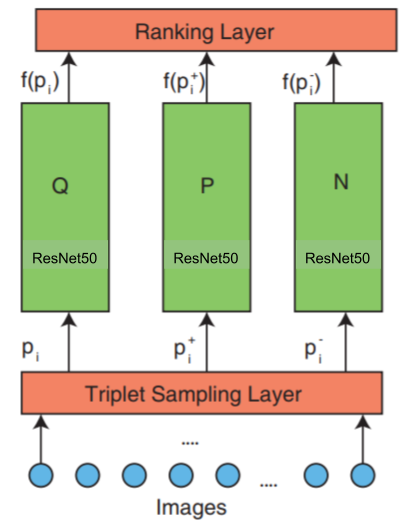
\includegraphics[scale=0.5]{imgs/architecture.png}}
    \caption{Network architecture of Deep Ranking}
    \label{fig:architecture}
\end{figure}